%% - Foto do circuíto (Como resultado)
%% - Explicação de como a caixa foi feita (madeira), pintura (preta), adesivos ~ (Enfim, a metodologia)
%% - Explicação das saídas USBS (do porquê nós utilizamos ((porque são mais universais)), das cores dos leds de cada saída (Azul: 12V, Verde: 9V, Laranja: 5V)

\begin{figure}[h]
    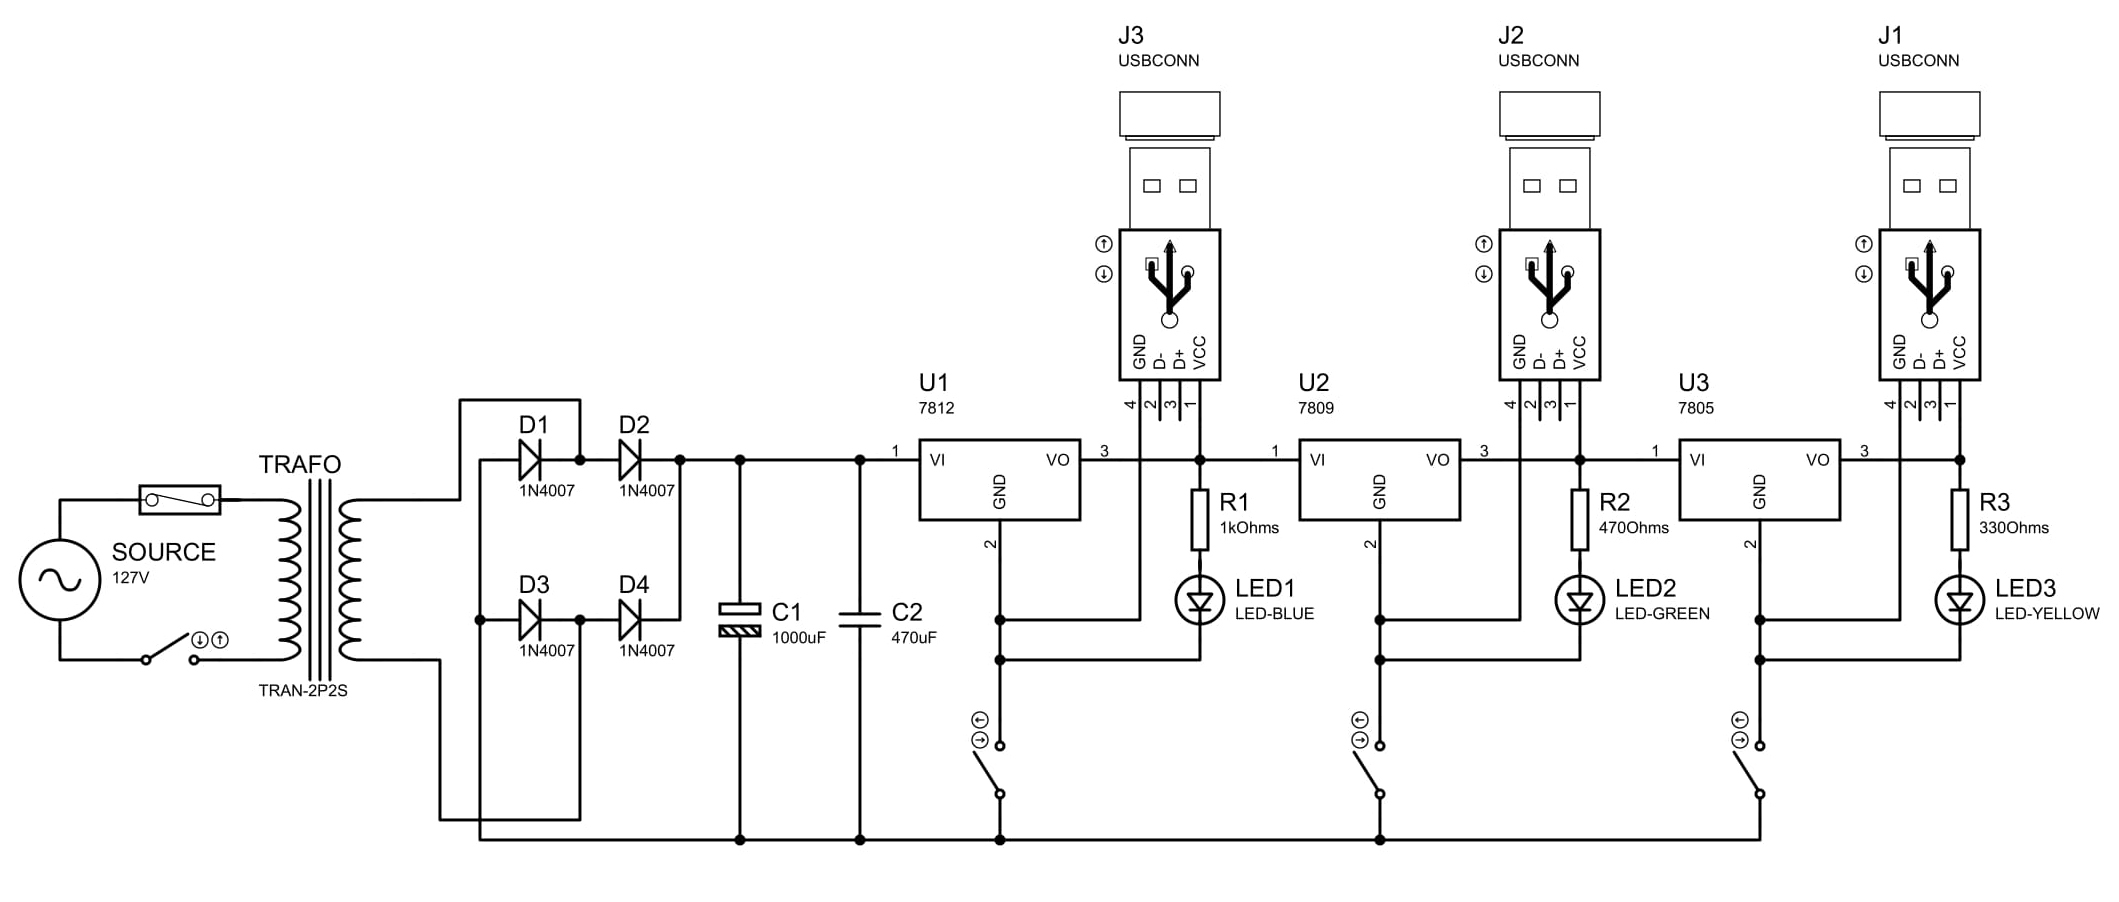
\includegraphics[height=7cm]{circuit-sketch}
    \caption{Desenho do Circuito Final}
    \label{fig:my_label}
\end{figure}

\par
A caixa na qual o circuito na placa universal foi comportada, é feita de madeira. Foram furados buracos correspondentes às saídas USB, os três LEDs (cada um acima de uma saída USB), furos para ventilar com ar externo e a entrada da energia AC. A caixa foi pintada com tinta da cor preta e adornada com adesivo contendo a logo e o nome do subprojeto.
\par
O motivo da utilização de saídas USB foi a universalidade, são mais comuns na atualidade para a função de fornecer energia à aparelhos eletrônicos como celulares, instrumentos musicais elétricos e \textit{modems}. Os LEDs de cores diferentes são úteis para diferenciar uma saída de outra. Todos esses aspectos proporcionam experiência simples para um usuário. O circuito representado na Figura 1 foi soldado na placa universal. \textit{Jumpers}, e até a própria solda em alguns casos, foram utilizados para estabelecer as conexões nos terminais positivos e negativos dos componentes.
\par
A primeira etapa do processo de conversão se situa na extremidade esquerda do circuito da Figura 1, a tensão que chegará através da tomada, podendo ser 110 volts ou 220 volts, será reduzida pelo transformador TRAN-2P2S para 18v, sendo ainda alternada. Em seguida, a regulagem da tensão é feita por diodos retificadores D1, D2, D3 e D4, transformando corrente alternada em contínua, apesar das oscilações. Depois disso é feita a filtragem capacitiva, utilizando os capacitores em paralelo, essa filtragem é capaz de estabilizar mais a corrente. Ainda sim exitem os chamados \textit{ripples}, que é uma pequena variação periódica residual da corrente contínua. Essa variação que ocorre a cada ciclo, é derivada dos tempos de carga e descarga dos capacitores. Já próximos às saídas, os reguladores de tensão linear mantém uma voltagem de saída constante.